\chapter{Revisiting SATzilla Features in 2024}\label{ch:ch03:rev_SATzilla}

\section{Introduction}





The Boolean satisfiability problem (\gls{sat}) is an important problem in computer science from both theoretical and practical viewpoints.
Common usages of \gls{sat} include hardware and software verification, cryptography, and more. 

However, as \gls{sat} is $\mathcal{NP}$-complete, it takes substantial time and computing power to solve it, which becomes prohibitively expensive as formulas become larger.

In order to deepen our understanding of \gls{sat} itself and develop better \gls{sat} solvers, it is of crucial importance to be able to describe \gls{sat} instances via an informative set of features.



Some of the most widely adopted such features are the SATzilla features~\cite{NudEtAl04,HutEtAl14}. 

These are a fixed set of features that are calculated from the DIMACS \gls{cnf} representation of a \gls{sat} instance. The SATzilla features consist of multiple groups, ranging from basic syntactic features describing the formula, such as its number of variables and clauses, to more complicated features, such as probing features derived from short runs of \gls{sat} solvers. Another type of features are based on statistics of graph representations of a given formula.

The SATzilla features have been successfully used in various domains, such as empirical performance models (\glspl{epm}; also known as performance or running time prediction) and algorithm selection~\cite{XuEtAl08,XuEtAl12}, algorithm configuration~\cite{HutEtAl11}, and benchmark generation~\cite{LeyEtAl09}. 

The features are also used for caching in CDCL-based model counting solvers~\cite{RooEtAl21} and in a variety of \gls{sat} solvers that incorporate machine learning techniques~\cite{GuoEtAl23}
However, the SATzilla features in their latest version date back to 2012. 

Since then, the \gls{sat} community has undergone various changes.
Most notably, \gls{sat} instances that we typically encounter today have a larger number of variables and clauses, thus taking significantly more time and memory to preprocess. Currently, the existing SATzilla feature extraction tool is unable to compute many of these features because of time and memory limitations.


In this paper, we revisit the SATzilla features and introduce a new version of the feature extraction tool. First, we replace the underlying solvers and the preprocessor with their most up-to-date versions. We then fix compilation errors and other memory errors related to dealing with larger formulas. Finally, we allow the user to set the time limits for feature computation. 
We compare the performance of our new tool with the old one in two \gls{sat} competitions. We measure the running times and the number of extracted features to check for performance gains of our new tool. We then evaluate the extracted features on three downstream tasks: satisfiability prediction, performance prediction and algorithm selection. We show that our new tool yields an important advantage in performance compared to the old tool across all three tasks.

The rest of the paper is organised as follows. We give a historical overview of the development and applications of the SATzilla features in~\cref{sec:ch03:related-work}. We then introduce the technical definitions, as well as the standard methodological pipeline in~\cref{sec:ch03:SATzilla-features}, wrapping it up with the contributions of this study. The results are presented in~\cref{sec:ch03:experiments}, and conclusions drawn in~\cref{sec:ch03:conclusions}.

\section{Related work}
\label{sec:ch03:related-work}












The SATzilla features were first introduced by Nudelman~et~al.~\cite{NudEtAl04} to construct \glspl{epm}, \emph{i.e.}, machine learning models that predict the running time of various \gls{sat} solvers given the features representing \gls{sat} instances. The authors identified key features that contribute the most towards having a good \gls{epm} prediction.

Consequently, they used the \glspl{epm} as a basis for algorithm selection, in which the algorithm that is selected corresponds to the one with the lowest predicted running time. 

They leveraged the \textit{performance complementarity} phenomenon of \gls{sat} solvers, where no \gls{sat} solver dominates all others over all instances. 
Therefore, selecting the best solver for each instance results in substantially better performance compared to choosing any standalone solver for all instances.
The SATzilla features were also successfully used for the satisfiability prediction task for \gls{sat} instances from various distributions~\cite{DevOSu08}. 



Further developments in algorithm selection led to the 2007 version of the SATzilla algorithm selector~\cite{XuEtAl08}, which combined running time and satisfiability prediction with other improvements. It won multiple medals in the \gls{sat} competition. This shows that extracting features from \gls{sat} instances can also speed up the solving process, and not only help understanding \gls{sat}. A newer version of the SATzilla algorithm selector was introduced in 2012~\cite{XuEtAl12}, winning multiple awards as well. It used a random forest as a predictor, and introduced an ensemble of pairwise classifiers to establish a ranking of the solvers, instead of predicting the running times directly. Additional features were introduced thereafter, revealing further important information about \gls{sat} instances. 




Another common usage of the SATzilla features is (model-based) algorithm configuration. To this end, the hyperparameters of \gls{sat} solvers are optimised such that their performance is as good as possible on all instances. As running \gls{sat} solvers is computationally expensive, a surrogate model is employed; it takes as an input a configuration of hyperparameters and instance features and predicts the performance of the \gls{sat} solver using a given configuration on a given instance. The instance features boost the accuracy of the surrogate model. An example of that is SMAC~\cite{HutEtAl11}, which successfully used the SATzilla features to optimise the performance of a wide range of \gls{sat} solvers on various benchmarks.


Last but not least, feature-based \glspl{epm} are proven to be useful for benchmark generation~\cite{LeyEtAl09}. In this context, given a new instance, we compute the features, which is usually cheaper than running a \gls{sat} solver, and use the \gls{epm} to predict whether the instance is hard (or not) for the solvers at hand.






















\section{SATzilla features}
\label{sec:ch03:SATzilla-features}


The SATzilla features describe the \gls{sat} formula using various representations and statistics. We briefly introduce three graph representations of a \gls{sat} formula, as undirected graphs are a meaningful representation of \gls{sat}, maintaining the permutation invariance: a) variable graph: nodes are variables, an edge exists if variables appear in the same clause; b) clause graph: nodes are clauses, an edge exists when two clauses share a negated literal; and c) variable-clause graph: nodes are variables and clauses, an edge exists between a variable node and a clause node if the variable appears in the clause.



Feature computation starts with the \emph{preprocessing} of the formula. This step, performed before solving an instance, renders the formula more accessible for \gls{sat} solvers. This means that the features are also computed on the version of the formula that is close to the one seen by the solvers. We believe that all these aspects can be boosted by using a modern preprocessor.
Features are classically computed using the \textsc{SATElite} preprocessor. We instead use the SBVA preprocessor, suggested by the winning solver from the 2023 \gls{sat} Competition. SBVA is also able to terminate after a set cutoff time, allowing for partial preprocessing, while \textsc{SATElite} does not include this functionality.
The preprocessed formula can then be directly used by a \gls{sat} solver without additional preprocessing within the solver, which improves the performance of algorithm selection.







Following the preprocessing, the \emph{feature extraction} begins. There are ten feature groups that can be extracted. We note that we describe the feature groups according to their implementation in the SATzilla feature extraction tool, not according to their definitions from the corresponding paper~\cite{HutEtAl14}. We point out that all feature groups include the time required to compute the features in the group.


\noindent\textbf{Preliminary} features include the number of variables and clauses before/after preprocessing. The running time of this feature group includes the preprocessing time and the time required to read the formula. \changed{This group contains 7 features.}

\noindent\textbf{Basic} features are cheap features that provide a basic description of the formula. They consist of the variable-clause ratio, the ratio between positive and negative literals in each clause, the number of unary, binary and ternary clauses, as well as statistics on clause nodes in the variable-clause graph. \changed{This group contains 15 features.}

\noindent\textbf{KLB} are expensive features that include the node degree statistics of the variable nodes in the variable-clause graph, and the ratio of positive to negative occurrences of each variable. They also include measures for the proximity to Horn formula, such as the fraction of Horn clauses and statistics on the number of times each variable appears in a Horn clause. \changed{This group contains 21 features.}

\noindent\textbf{Clause graph} (\gls{clg}) features are expensive features that contain statistics on the degree of the nodes in the clause graph, as well as the clustering coefficient. \changed{This group contains 11 features.}

\noindent\textbf{Diameter} features contain information on the diameter of the variable graph, which is the shortest path between each pair of nodes in the graph. \changed{This group contains 6 features.}

\noindent\textbf{\gls{dpll} probing} (or unit propagation) features are computed by running the \gls{dpll} algorithm for various depths and measuring the number of unit propagations at each depth. \changed{This group contains 6 features.}

\noindent\textbf{Lobjois} features are an estimation of the size of the search space. They are computed by running the \gls{dpll} algorithm multiple times until a contradiction is found. Then, the average depth of the contradictions is the log-estimation of the search space. 

\changed{This group contains 3 features, which are all based on the work of Lobjois and Lema\^{\i}tre~\cite{LobLem98}.}

\noindent\textbf{Survey propagation} features are based on computing statistics on the following probabilities returned by the VARSAT \cite{HsuMcI09} solver: a probability of each variable to be assigned to True, to False, and to be unconstrained. \changed{This group contains 19 features.}

    
\noindent\textbf{Clause learning} (CL) features are based on running a CDCL solver (ZChaff rand~\cite{MahEtAl04} in the 2012 version, CadiCal~\cite{BieEtAl20} in our new version) for two seconds. We measure the number and length of learned clauses for every 1000 decisions, and compute the statistics of those values. \changed{This group contains 19 features.}

\noindent\textbf{Local search} (LS) features are obtained by running two local search solvers many times, each time up to 10000 steps, and computing statistics on those runs. In the 2012 version, the local search solvers are GSAT and \gls{saps}. We instead use GSAT and Sparrow 2011 in our new version. \changed{This group contains 24 features.}

\noindent\textbf{Linear programming} (LP) features are based on solving a relaxed version of the \gls{sat} formula, 

where $C_1\land C_2\land \dots \land C_N$ is a Boolean formula \changed{with $N$ \gls{cnf} clauses $C_1 \ldots C_N$ over Boolean variables $x_j$. We now consider linear programming variables $x_j$ and
solve the following linear programming problem:
Maximise
    $\sum_{i=1}^N \sum_{l\in C_i} v(l)$, 
where the value $v(l)$ of literal $l$ is defined as $v(x_j)=x_j$, $v(\neg x_j)=1-x_j$, 
    while keeping
    $\sum_{l\in C_i} v(l) \geq 0$ 
    for each $C_i$ and $0 \leq x_j \leq 1$ for each $x_j$. 
    This means that every variable has a value between 0 and 1, each clause has a value which is the sum of values of all literals, and the value of the formula is the sum of values of all clauses. The goal is to maximise the value of the formula, while keeping the value of every clause positive. Finally, statistics on the linear programming solution are extracted. In the new version, we upgrade the linear programming solver package, lp solve. This group contains 7 features.}



We note that the basic, KLB and clause graph features are computed sequentially, with each feature group being dependent on the successful computation of the previous groups; \emph{e.g.}, if the computation of the basic features fails, the KLB and clause graph features will not be computed at all.

Another change we applied to the feature extraction tool is allowing a more precise timeout setting. In the 2012 version, the time limits were hard-coded and set to high values (for example, 1200 seconds for preprocessing). This can cause many feature computations to simply terminate without computing any features at all. To this end, we adjust the code in the new version to allow the user to set the time limits through a command line argument.

\section{Experiments}
\label{sec:ch03:experiments}
We evaluate our new SATzilla feature extraction tool on the formulas stemming from two latest (2022 and 2023) \gls{sat} Competitions. We first look at the feature extraction times and then evaluate the features on three downstream tasks: satisfiability prediction, running time prediction, and algorithm selection.

To assess the advantage of using the new version of the extraction tool, we extract the features using both our new version and the 2012 version of the tool, with a time limit of 180 seconds per feature group. 

We use a cluster of 18 nodes, each equipped with 2 AMD EPYC 7543 32-core CPUs with 256 MB L3 cache. Each node also has 1TB of memory. The cluster is running on a Rocky Linux 9.4 operating system. We measure running times using the runsolver tool \cite{Roussel11c}.

\subsection{Feature computation time}
\label{sec:ch03:feature-computation-time}

\begin{figure*}[h]
    \caption[Percentage of computed features (2022 SAT Competition)]{Percentage of features computed by the old tool (SATzilla 2012; in red) and the new tool (SATzilla 2024; in blue) over the available time budget for each feature group on the 2022 \gls{sat} Competition. For most feature groups, the new tool extracts features from more instances than the old one.}
    \centering
    \begin{subfigure}[b]{0.24\textwidth}
        \centering
        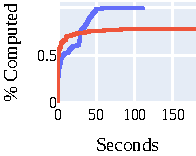
\includegraphics[]{figures/03/figs/ecdf_sc2022_Pre-featuretime.pdf}
        \caption{Preliminary}
        \label{fig:ch03:satcomp22_pre}
    \end{subfigure}
    \centering
    \begin{subfigure}[b]{0.24\textwidth}
        \centering
        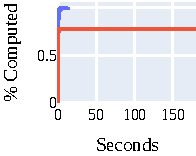
\includegraphics[]{figures/03/figs/ecdf_sc2022_Basic-featuretime.pdf}
        \caption{Basic}
        \label{fig:ch03:satcomp22_basic}
    \end{subfigure}
    \begin{subfigure}[b]{0.24\textwidth}
        \centering
        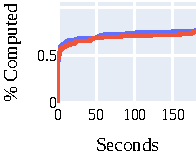
\includegraphics[]{figures/03/figs/ecdf_sc2022_KLB-featuretime.pdf}
        \caption{KLB}
        \label{fig:ch03:satcomp22_klb}
    \end{subfigure}
        \begin{subfigure}[b]{0.24\textwidth}
        \centering
        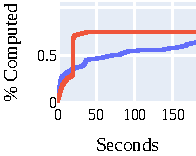
\includegraphics[]{figures/03/figs/ecdf_sc2022_CG-featuretime.pdf}
        \caption{Clause graph}
        \label{fig:ch03:satcomp22_cg}
    \end{subfigure}
    \centering
    \begin{subfigure}[b]{0.24\textwidth}
        \centering
        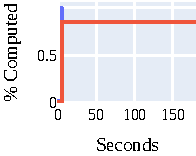
\includegraphics[]{figures/03/figs/ecdf_sc2022_cl-featuretime.pdf}
        \caption{Clause learning}
        \label{fig:ch03:satcomp22_cl}
    \end{subfigure}
    \begin{subfigure}[b]{0.24\textwidth}
        \centering
        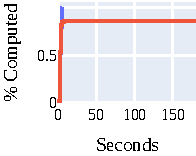
\includegraphics[]{figures/03/figs/ecdf_sc2022_ls-gsat-featuretime.pdf}
        \caption{LS: GSAT}
        \label{fig:ch03:satcomp22_ls_gsat}
    \end{subfigure}
        \begin{subfigure}[b]{0.24\textwidth}
        \centering
        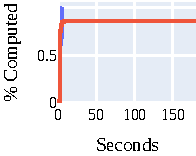
\includegraphics[]{figures/03/figs/ecdf_sc2022_ls-saps-featuretime.pdf}
        \caption{LS: \gls{saps}/Sparrow}
        \label{fig:ch03:satcomp22_ls_saps}
    \end{subfigure}
    \centering
    \begin{subfigure}[b]{0.24\textwidth}
        \centering
        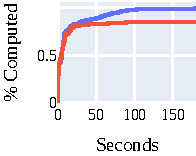
\includegraphics[]{figures/03/figs/ecdf_sc2022_sp-featuretime.pdf}
        \caption{Survey propagation}
        \label{fig:ch03:satcomp22_sp}
    \end{subfigure}
    \begin{subfigure}[b]{0.24\textwidth}
        \centering
        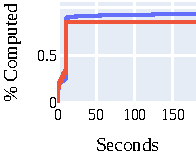
\includegraphics[]{figures/03/figs/ecdf_sc2022_DIAMETER-featuretime.pdf}
        \caption{Diameter}
        \label{fig:ch03:satcomp22_dia}
    \end{subfigure}
    \begin{subfigure}[b]{0.24\textwidth}
        \centering
        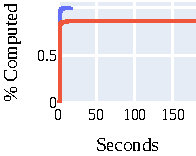
\includegraphics[]{figures/03/figs/ecdf_sc2022_lobjois-featuretime.pdf}
        \caption{Lobjois}
        \label{fig:ch03:satcomp22_lobjois}
    \end{subfigure}
    \begin{subfigure}[b]{0.24\textwidth}
        \centering
        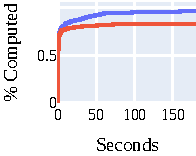
\includegraphics[]{figures/03/figs/ecdf_sc2022_unit-featuretime.pdf}
        \caption{Unit propagation}
        \label{fig:ch03:satcomp22_unit}
    \end{subfigure}
    \begin{subfigure}[b]{0.24\textwidth}
        \centering
        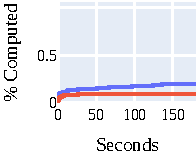
\includegraphics[]{figures/03/figs/ecdf_sc2022_lpTIME.pdf}
        \caption{Linear programming}
        \label{fig:ch03:satcomp22_lp}
    \end{subfigure}
    \label{fig:ch03:feat_comtimes_2022}
\end{figure*}

\begin{figure*}[h]
    \caption[Percentage of computed features (2023 SAT Competition)]{Percentage of features computed by the old tool (SATzilla 2012; in red) and the new tool (SATzilla 2024; in blue) over the available time budget for each feature group on the 2023 \gls{sat} Competition. For most feature groups, the new tool extracts features from more instances than the old one.}

    \begin{subfigure}[b]{0.24\textwidth}
        \centering
        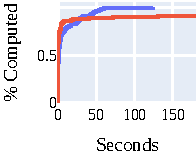
\includegraphics[]{figures/03/figs/ecdf_sc2023_Pre-featuretime.pdf}
        \caption{Preliminary}
        \label{fig:ch03:satcomp23_pre}
    \end{subfigure}
    \centering
    \begin{subfigure}[b]{0.24\textwidth}
        \centering
        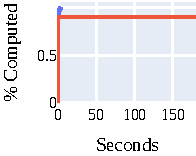
\includegraphics[]{figures/03/figs/ecdf_sc2023_Basic-featuretime.pdf}
        \caption{Basic}
        \label{fig:ch03:satcomp23_basic}
    \end{subfigure}
    \begin{subfigure}[b]{0.24\textwidth}
        \centering
        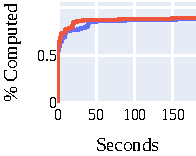
\includegraphics[]{figures/03/figs/ecdf_sc2023_KLB-featuretime.pdf}
        \caption{KLB}
        \label{fig:ch03:satcomp23_klb}
    \end{subfigure}
        \begin{subfigure}[b]{0.24\textwidth}
        \centering
        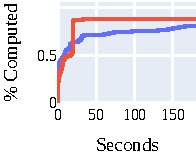
\includegraphics[]{figures/03/figs/ecdf_sc2023_CG-featuretime.pdf}
        \caption{Clause graph}
        \label{fig:ch03:satcomp23_cg}
    \end{subfigure}
    \centering
    \begin{subfigure}[b]{0.24\textwidth}
        \centering
        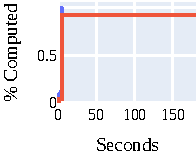
\includegraphics[]{figures/03/figs/ecdf_sc2023_cl-featuretime.pdf}
        \caption{Clause learning}
        \label{fig:ch03:satcomp23_cl}
    \end{subfigure}
    \begin{subfigure}[b]{0.24\textwidth}
        \centering
        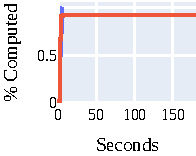
\includegraphics[]{figures/03/figs/ecdf_sc2023_ls-gsat-featuretime.pdf}
        \caption{LS: GSAT}
        \label{fig:ch03:satcomp23_ls_gsat}
    \end{subfigure}
        \begin{subfigure}[b]{0.24\textwidth}
        \centering
        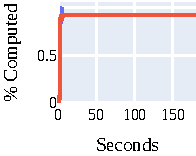
\includegraphics[]{figures/03/figs/ecdf_sc2023_ls-saps-featuretime.pdf}
        \caption{LS: \gls{saps}/Sparrow}
        \label{fig:ch03:satcomp23_ls_saps}
    \end{subfigure}
    \centering
    \begin{subfigure}[b]{0.24\textwidth}
        \centering
        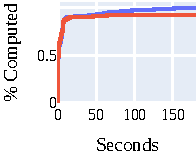
\includegraphics[]{figures/03/figs/ecdf_sc2023_sp-featuretime.pdf}
        \caption{Survey propagation}
        \label{fig:ch03:satcomp23_sp}
    \end{subfigure}
    \begin{subfigure}[b]{0.24\textwidth}
        \centering
        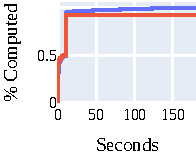
\includegraphics[]{figures/03/figs/ecdf_sc2023_DIAMETER-featuretime.pdf}
        \caption{Diameter}
        \label{fig:ch03:satcomp23_dia}
    \end{subfigure}
    \begin{subfigure}[b]{0.24\textwidth}
        \centering
        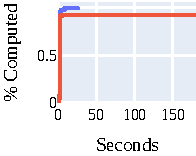
\includegraphics[]{figures/03/figs/ecdf_sc2023_lobjois-featuretime.pdf}
        \caption{Lobjois}
        \label{fig:ch03:satcomp23_lobjois}
    \end{subfigure}
    \begin{subfigure}[b]{0.24\textwidth}
        \centering
        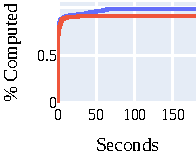
\includegraphics[]{figures/03/figs/ecdf_sc2023_unit-featuretime.pdf}
        \caption{Unit propagation}
        \label{fig:ch03:satcomp23_unit}
    \end{subfigure}
    \begin{subfigure}[b]{0.24\textwidth}
        \centering
        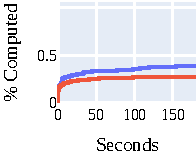
\includegraphics[]{figures/03/figs/ecdf_sc2023_lpTIME.pdf}
        \caption{Linear programming}
        \label{fig:ch03:satcomp23_lp}
    \end{subfigure}
    \label{fig:ch03:feat_comtimes_2023}
\end{figure*}

\cref{fig:ch03:feat_comtimes_2022,fig:ch03:feat_comtimes_2023} show the percentage of features computed over the available time budget using the old (depicted in red) and new (depicted in blue) SATzilla tool on the 2022 and 2023 \gls{sat} Competition data, respectively. For simplicity, due to the similarity of the overall results between the two competitions, we draw more detailed insights based on plots from the 2023 edition (\cref{fig:ch03:feat_comtimes_2023}). 

We first observe that the new tool is able to extract more features than the old one for most feature groups. In particular, we highlight the performance gains on the preliminary feature group (\cref{fig:ch03:satcomp23_pre}), for which the new tool can extract the features for all formulas, compared to less than $80\%$ of the formulas when using the the old tool. We note that for some feature groups, like graph learning (\cref{fig:ch03:satcomp23_cg}), the old tool is able to extract more features compared to the preliminary feature group. This is due to the fact that the old tool extracts the preliminary, basic, KLB and \gls{clg} feature groups together. Therefore, in case computing one of those groups takes a long time, the whole feature extraction fails.

We also note that for KLB and \gls{clg} features there is an advantage for the old version, due to the new SBVA preprocessing method yielding larger formulas than its predecessor \textsc{SATElite} (as in many cases smaller formulas are not always easier to solve). Similarly, the expensive graph-based features (\emph{e.g.}, \cref{fig:ch03:satcomp23_cg,fig:ch03:satcomp23_dia}) require more time to extract than smaller formulas. 

\changed{This is more apparent in the 2022 \gls{sat} Competition, where larger instances were used than in the 2023 \gls{sat} Competition.}




\subsection{Satisfiability prediction}
\label{sec:ch03:satisfiability-prediction}

The first downstream task is satisfiability prediction, for which we measure the performance when using features extracted by our tool. 

We use the random forest (RF) classifier from the scikit-learn package to learn the mapping between features (representing \gls{sat} instances) and outputs (satisfiable or unsatisfiable). We optimise the hyperparameters of the RF for one hour using SMAC3~\cite{LinEtAl22b} on 10-fold cross-validation of the training data.
We consider instances from the 2022 and 2023 \gls{sat} Competitions for which we know the satisfiability result (put differently, we omit instances for which the solution is unknown). On each competition, we evaluate the performance of the RF model using 10-fold cross-validation. This results in having outer cross-validation (for evaluation) and inner cross-validation (for training). Such techniques have been previously used by AutoFolio~\cite{LinEtAl15}.

We present the satisfiability prediction accuracy scores in \cref{fig:ch03:sat_prediction}. We see that, by using features extracted via the new tool, we achieve better performance across all instances on both \gls{sat} competitions. Furthermore, we notice that the new tool leads to a higher accuracy gain for satisfiable instances than for unsatisfiable instances. For the latter, the accuracy remains very similar to the one achieved by using the old tool in the 2023 \gls{sat} Competition and slightly dropped for the 2022 \gls{sat} Competition. This might be due to the fact that the unsatisfiable instances are larger on average, thus being more prone to timeouts even when using our new tool, \changed{which goes along with the worse performance in the 2022 \gls{sat} Competition, where the unsatisfiable instances were larger than in the 2023 \gls{sat} Competition}. We point out that such high accuracy was already achieved before for industrial \gls{sat} instances~\cite{DevOSu08}.


\begin{figure*}[h]
    \caption[Satisfiability prediction accuracy]{Accuracy of the satisfiability prediction task using a random forest with features extracted by the old (SATzilla 2012) and the new tool (SATzilla 2024). We see an overall higher accuracy for the new tool, which results from higher accuracy on satisfiable instances. On unsatisfiable ones, the accuracy remains the same.}
    \label{fig:ch03:sat_prediction}
    \begin{subfigure}[b]{0.49\textwidth}
        \centering
        

        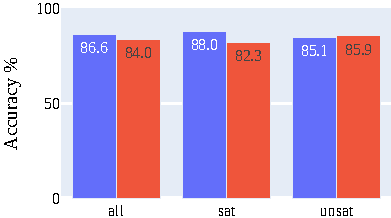
\includegraphics[]{figures/03/figs/sat_bar_2022.pdf}
        \caption{2022 \gls{sat} Competition}
        \label{fig:ch03:satpred22}
    \end{subfigure}
    \centering
    \begin{subfigure}[b]{0.49\textwidth}
        \centering
        

        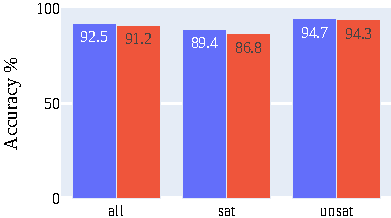
\includegraphics[]{figures/03/figs/sat_bar_2023.pdf}
        \caption{2023 \gls{sat} Competition}
        \label{fig:ch03:satpred23}
    \end{subfigure}
\end{figure*}


\subsection{Performance prediction}
The second downstream task we investigate is performance prediction, which has important applications in algorithm selection, configuration and benchmark generation. We refer to the methodology described in~\cite{HutEtAl14} and use a RF regressor as the \gls{epm}. It is important to note that for an accurate running time prediction we need to perform a $log_{10}$ transformation of running times prior to training the model, as done by Hutter 
\emph{et al.}~\cite{HutEtAl14}. This transformation allows to capture the order of magnitude rather than small variations in the running time. The \gls{epm} then maps instance features to the log-transformed running times, and we aim to minimise the root mean squared error (\gls{rmse}) of the model, which is defined as $\sqrt{\frac{1}{n}\cdot \sum_{i=1}^n (\hat{y}_i-y_i)^2}$ for $n$ predicted running times  $\hat{y}_i$ and ground truth running times  $y_i$. Lower \gls{rmse} scores are better and 0 is the optimal value.
In line with the previous task, we perform inner and outer cross-validation and optimise the RF's hyperparameters for one hour using SMAC3.

We look into the performance of the \gls{epm} for running time prediction on all solvers from the 2022 and 2023 \gls{sat} Competitions. Here, we do not actually run solvers on instances to record their running times, but rather use the running times reported by the competitions. We display the results for the 10 best solvers from each competition in \cref{fig:ch03:rt_pred} (the results for all solvers can be found in the supplementary material). We see that using the features extracted by the new tool leads to the lower \gls{rmse} for all solvers, compared to using those extracted by the old tool. For some solvers, we observe a significantly lower \gls{rmse}, like Kissat{\_}MAB{\_}prop-no{\_}sym, where using the new tool decreases the \gls{rmse} from 0.84 to 0.69. \cref{fig:ch03:rmse_hists} shows the histogram of the error percentage for all solvers in the 2022 and 2023 \gls{sat} Competitions. We see that for the 2022 competition, the new tool has more instances with error rate lower than $10\%$ compared to the old version. For the 2023 competition, using the features extracted with the new version, more instances are predicted with less than $1\%$ error. Histograms per solver are available in \cref{sec:rts_hists_per_solver}.

\begin{figure*}[h]
    \caption[RMSE of running time prediction]{Root mean square error (\gls{rmse}) of (log-transformed) running time prediction using a random forest with features extracted by the old (SATzilla 2012; in red) and the new tool (SATzilla 2024; in blue), on \gls{sat} solvers from the 2022 and 2023 \gls{sat} Competitions. The new tool achieves lower \gls{rmse} for all solvers.}
    \label{fig:ch03:rt_pred}
    \begin{subfigure}[b]{0.99\textwidth}
        \centering
        
        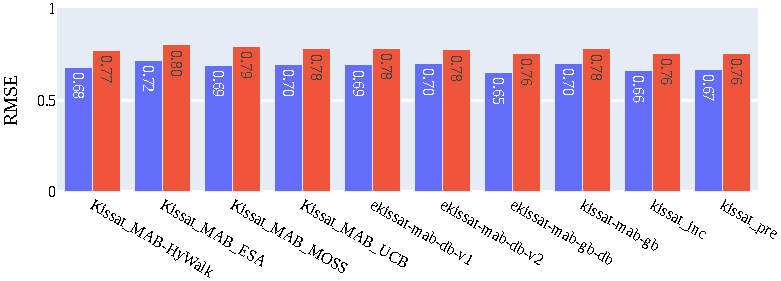
\includegraphics[]{figures/03/figs/rts_bar_2022.pdf}
        \caption{2022 \gls{sat} Competition}
        \label{fig:ch03:rt_pred22}
    \end{subfigure}
    \centering
    \begin{subfigure}[b]{0.99\textwidth}
        \centering
        
        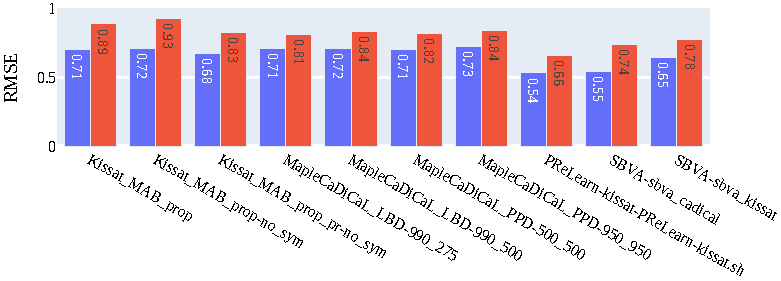
\includegraphics[]{figures/03/figs/rts_bar_2023.pdf}
        \caption{2023 \gls{sat} Competition}
        \label{fig:ch03:rt_pred23}
    \end{subfigure}
\end{figure*}


\begin{figure*}[h]
    \caption[Error percentage histogram of running time prediction]{Histogram of the error percentage of the root mean square error (\gls{rmse}) of (log-transformed) running time prediction using a random forest with features extracted by the old (SATzilla 2012; in red) and the new tool (SATzilla 2024; in blue), on \gls{sat} solvers from the 2022 and 2023 \gls{sat} Competitions. The new tool achieves lower error percentages.}
    \label{fig:ch03:rmse_hists}
    \begin{subfigure}[b]{0.49\textwidth}
        \centering
                

        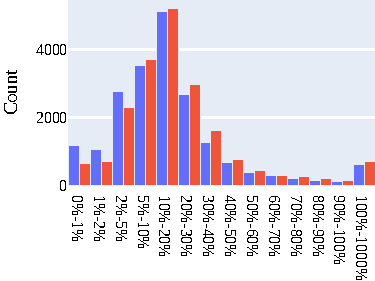
\includegraphics[]{figures/03/figs/acc_rt_pred_sc2022_both.pdf}
        \caption{2022 \gls{sat} Competition}
        \label{fig:ch03:rmse_hist_2022}
    \end{subfigure}
    \centering
    \begin{subfigure}[b]{0.49\textwidth}
        \centering
        

        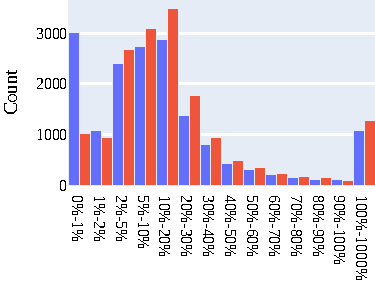
\includegraphics[]{figures/03/figs/acc_rt_pred_sc2023_both.pdf}
        \caption{2023 \gls{sat} Competition}
        \label{fig:ch03:rmse_hist_2023}
    \end{subfigure}
\end{figure*}

































\subsection{Algorithm selection}
The third and final downstream task we consider is algorithm selection. In algorithm selection, given a set of instances $I$, a set of solvers (\emph{i.e.}, algorithm portfolio) $\mathbf{A}$ and a performance metric $m: \mathbf{A} \times I \rightarrow \mathbb{R}$, we build an algorithm selector $S: I \rightarrow \mathbf{A}$ such that its performance is optimal on the instance set $I$ according to the metric $m$.
We compare the performance of algorithm selection to two standard baselines, the single best solver (\gls{sbs}; \emph{i.e}, the solver with the lowest overall running time) and the virtual best solver (\gls{vbs}; \emph{i.e.}, the theoretical oracle which for each instance selects the actual best solver on it).

We measure the performance of algorithm selection using \textit{closed gap}, which is computed as $\frac{m_{\gls{sbs}} - m_{S}}{m_{\gls{sbs}} - m_{\gls{vbs}}}$, (\emph{i.e.}, the closed gap stands for how much of the gap between the \gls{sbs} and the \gls{vbs} is closed by using the algorithm selector).
We then use AutoFolio~\cite{LinEtAl15} as an algorithm selector, which consists of multiple algorithm selection approaches, from which the best one is suggested by using algorithm configuration.


As algorithm portfolio for the selection, we use the 10 best solvers from each \gls{sat} competition. We train the selector for 8 hours.

\cref{fig:ch03:closed_gap} shows the closed gap results on the 2022 and 2023 \gls{sat} Competitions. Positive closed gap values on both scenarios using both the old and the new tool indicate that, in general, SATzilla features are useful for the algorithm selection task. 

Importantly, features extracted with the new tool lead to better closed gap values on both scenarios.

In \cref{fig:ch03:ecdf_as}, we provide ECDF plots showing the fraction of instances solved over time. In the 2022 \gls{sat} Competition scenario, the old version of the tool performs worse than the \gls{sbs} until a budget of approximately 1000 seconds, while the new version of the tool performs similarly to the \gls{sbs}. After 1000 seconds, both versions of the SATzilla features perform similarly. In the 2023 \gls{sat} Competition scenario, the new tool performs better than the old one for budgets between 100 and 1000 seconds. With a budget of less than 10 seconds, the old tool solves more instances. 

Overall, the ECDF plots reflect well what is shown in \cref{fig:ch03:closed_gap}, where we see that the new tool exhibits a few percents higher closed gap value.




\begin{figure}[h]
    \centering
    \caption[Closed gap values for algorithm selection]{Closed gap values for the algorithm selection task using the old (SATzilla 2012; in red) and the new tool (SATzilla 2024; in blue) on the 2022 and 2023 \gls{sat} Competitions; higher is better.}
    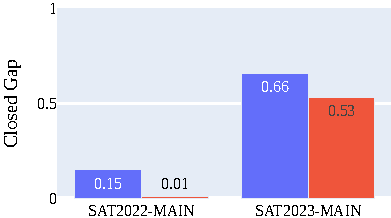
\includegraphics{figures/03/figs/as_bar_2023.pdf}
    \label{fig:ch03:closed_gap}
\end{figure}

\begin{figure*}[h]
    \caption[ECDF plots for algorithm selection]{ECDF plots for the algorithm selection task using the old (SATzilla 2012) and the new tool (SATzilla 2024) on the 2022 and 2023 \gls{sat} Competitions.}
    \label{fig:ch03:ecdf_as}
    \begin{subfigure}[b]{0.49\textwidth}
        \centering
        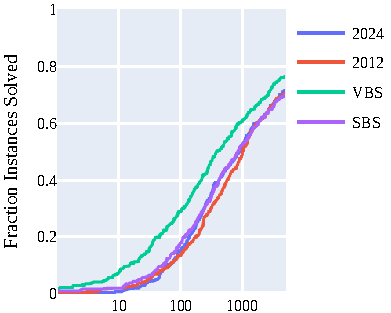
\includegraphics[]{figures/03/figs/ecds_af_2022.pdf}
        \caption{2022 \gls{sat} Competition}
        \label{fig:ch03:ecdf_as_2022}
    \end{subfigure}
    \centering
    \begin{subfigure}[b]{0.49\textwidth}
        \centering
        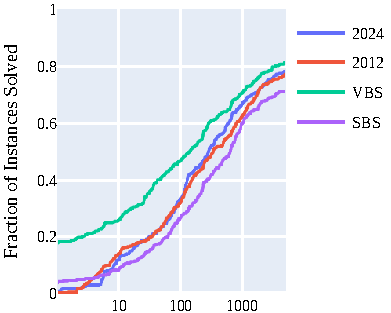
\includegraphics[]{figures/03/figs/ecds_af_2023.pdf}
        \caption{2023 \gls{sat} Competition}
        \label{fig:ch03:ecdf_as_2023}
    \end{subfigure}
\end{figure*}




































\section{Chapter conclusion}
\label{sec:ch03:conclusions}

This chapter introduced an improved version of the well-known SATzilla feature extraction tool, motivated by the need to make feature extraction more robust through better user infrastructure and bug fixes.
The new version uses up-to-date preprocessing techniques and \gls{sat} solvers, which allow for better representation of \gls{sat} formulae.
The experiments showed that the new tool improves satisfiability prediction, reduces error for running time prediction, and achieves a better closed gap for algorithm selection.

The SATzilla 2024 extraction tool aims to facilitate and promote the use of \gls{sat} features even beyond their current scope.
It is easily extensible and thus supports future work on new features, for example features based on recent developments in the explainability of \gls{sat} solvers~\cite{ElfEtAl18}, or other advancements in \gls{sat}.

\paragraph{Connection to the thesis}~
This chapter shows that empirical performance prediction can fail before modelling even begins if the underlying features are outdated, brittle, or too expensive to compute.
Modernising the SATzilla feature extractor therefore establishes the first thesis theme: better predictions require better access to reliable representations.
The next chapter broadens this representation question from \gls{sat} features to high-dimensional machine learning and black-box optimisation spaces.
